%%%%%%%%%%%%%%%%%%%%%%%%%%%%%%%%%%%%%%%%%%%%%%%%%%%%%%%%%%%%%%%%%%%%%%%%
%%%  THIS TEX FILE IS TO GENERATE PDF FILE FOR 
%%%     DATA MINING HOMEWORK 03
%%%  COPYRIGHT (C) JIMMY LIN, 2013, UT AUSTIN
%%%%%%%%%%%%%%%%%%%%%%%%%%%%%%%%%%%%%%%%%%%%%%%%%%%%%%%%%%%%%%%%%%%%%%%%
\documentclass[11pt,a4paper]{article}
%%%%%%%%%%%%%%%%%%%%%%%%%%%%%%%%%%%%%%%%%%%%%%%%%%%%%%%%%%%%%%%%%%%%%%%%
%%%  PACKAGES USED IN THIS TEX SOURCE FILE
%%%%%%%%%%%%%%%%%%%%%%%%%%%%%%%%%%%%%%%%%%%%%%%%%%%%%%%%%%%%%%%%%%%%%%%%
\usepackage{geometry,amsthm,amsmath,graphicx,fancyheadings,framed}
\usepackage{tikz}
\usepackage{fancybox}
\usepackage[]{./mcode}
\usetikzlibrary{automata,positioning}
\usepackage[colorlinks,
            linkcolor=blue,
            anchorcolor=red,
            citecolor=green
            ]{hyperref}
\usepackage{/Users/JimmyLin/workspace/latexTemplate/UTA_CS/JS}
\usepackage{/Users/JimmyLin/workspace/latexTemplate/UTA_CS/JSASGN}
%%%%%%%%%%%%%%%%%%%%%%%%%%%%%%%%%%%%%%%%%%%%%%%%%%%%%%%%%%%%%%%%%%%%%%%%
%%% MACROS CONTAINING THE FILE INFORMATION
%%%%%%%%%%%%%%%%%%%%%%%%%%%%%%%%%%%%%%%%%%%%%%%%%%%%%%%%%%%%%%%%%%%%%%%%
\renewcommand{\COURSE}{CS363D Statistical Learning and Data Mining}
\renewcommand{\LECTURER}{Pradeep Ravikumar}
\renewcommand{\TUTOR}{Adarsh Prasad}
\renewcommand{\TASK}{Homework 03}
\renewcommand{\RELEASEDATE}{March. 25 2014}
\renewcommand{\DUEDATE}{April. 07 2014}
\renewcommand{\TIMECONSUME}{7 hours}
%%%%%%%%%%%%%%%%%%%%%%%%%%%%%%%%%%%%%%%%%%%%%%%%%%%%%%%%%%%%%%%%%%%%%%%%
%%% DOCUMENTATION STARTS FROM HERE 
%%%%%%%%%%%%%%%%%%%%%%%%%%%%%%%%%%%%%%%%%%%%%%%%%%%%%%%%%%%%%%%%%%%%%%%%
\begin{document}
%%%%%%%%%%%%%%%%%%%%%%%%%%%%%%%%%%%%%%%%%%%%%%%%%%%%%%%%%%%%%%%%%%%%%%%%
%% TITLE PAGE
%%%%%%%%%%%%%%%%%%%%%%%%%%%%%%%%%%%%%%%%%%%%%%%%%%%%%%%%%%%%%%%%%%%%%%%%
\begin{titlepage}
    \maketitle
\end{titlepage}
%%%%%%%%%%%%%%%%%%%%%%%%%%%%%%%%%%%%%%%%%%%%%%%%%%%%%%%%%%%%%%%%%%%%%%%%
%% CONTENT PAGE: TABLEOFCONTENTS, LISTOFTABLES, LIST OF FIGURES
%%%%%%%%%%%%%%%%%%%%%%%%%%%%%%%%%%%%%%%%%%%%%%%%%%%%%%%%%%%%%%%%%%%%%%%%
\renewcommand{\contentsname}{Contents}
\begin{center} 
    \tableofcontents 
    %\listoftables 
    \listoffigures
\end{center}
\newpage
%%%%%%%%%%%%%%%%%%%%%%%%%%%%%%%%%%%%%%%%%%%%%%%%%%%%%%%%%%%%%%%%%%%%%%%%
%%% GENERAL DOCUMENTATION BEGINS 
%%%%%%%%%%%%%%%%%%%%%%%%%%%%%%%%%%%%%%%%%%%%%%%%%%%%%%%%%%%%%%%%%%%%%%%%

\newcommand{\uk}{\ensuremath{U^{(K_i)}}}
\newcommand{\ukt}{\ensuremath{U^{(K_i)^T}}}
\newcommand{\mk}{\ensuremath{M^{(K_i)}}}
\newcommand{\mkt}{\ensuremath{M^{(K_i)^T}}}
\section{MF Implementation}

\begin{figure}[h]
    \centering
    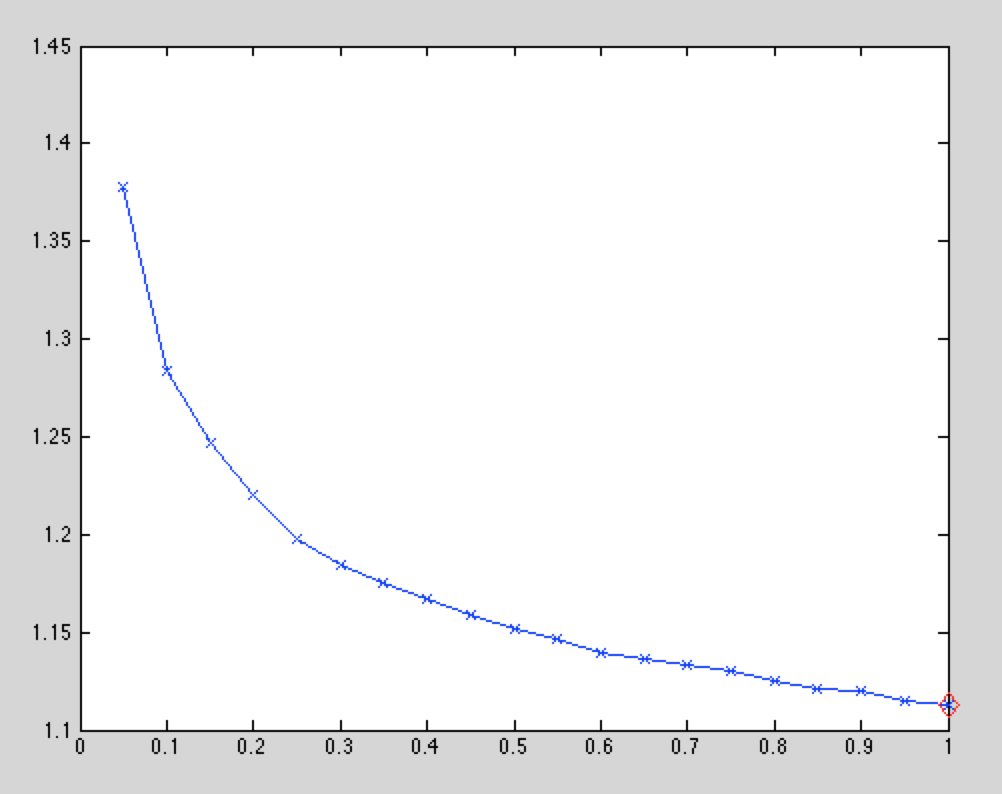
\includegraphics[width=5in,height=3.5in]{./lambda_error.png} \\
    \caption{Errors With Regard to Parameter $\lambda$}
\end{figure}
Note that the horizental axis represents the regularization parameter, and
vertical axis represents the RMSE on given regularization parameter. 

For specific details, see the source code in Appendix \ref{AppdendixA}.
For debugging, see the Execution logs in Appendix \ref{AppdendixB}.

\section{Report optimal $\lambda$}
The optimal lambda derived is $\lambda = 1$.

\section{Problem when $\lambda = 0$}
The problem encountered when $\lambda = 0$ is that the non-invertibility of
$\ukt * \uk$ and $\mkt * \mk$.


\section{RMSE of Test Set under optimal $\lambda$}
The RMSE of test set under optimal $\lambda = 1$ is $1.0835$.

\newpage
\appendix
\section{Source Code}
\label{AppdendixA}
\lstinputlisting{../solution.m}
\section{Execution Logs}
\label{AppdendixB}
\lstinputlisting{../logs.txt}

%%%%%%%%%%%%%%%%%%%%%%%%%%%%%%%%%%%%%%%%%%%%%%%%%%%%%%%%%%%%%%%%%%%%%%%%
%%% General Documentation ends
%%%%%%%%%%%%%%%%%%%%%%%%%%%%%%%%%%%%%%%%%%%%%%%%%%%%%%%%%%%%%%%%%%%%%%%%
\end{document}
